\documentclass{beamer}

%% Juego de caracteres usado en el archivo fuente: UTF-8
\usepackage{ucs}
\usepackage[utf8x]{inputenc}
\uselanguage{spanish}
%Para la identación del español
\usepackage[spanish]{babel}

% There are many different themes available for Beamer. A comprehensive
% list with examples is given here:
% http://deic.uab.es/~iblanes/beamer_gallery/index_by_theme.html
% You can uncomment the themes below if you would like to use a different
% one:
%\usetheme{AnnArbor}
%\usetheme{Antibes}
%\usetheme{Bergen}
%\usetheme{Berkeley}
%\usetheme{Berlin}
%\usetheme{Boadilla}
%\usetheme{boxes}
%\usetheme{CambridgeUS}
%\usetheme{Copenhagen}
%\usetheme{Darmstadt}
%\usetheme{default}
%\usetheme{Frankfurt}
%\usetheme{Goettingen}
%\usetheme{Hannover}
%\usetheme{Ilmenau}
%\usetheme{JuanLesPins}
%\usetheme{Luebeck}
\usetheme{Madrid}
%\usetheme{Malmoe}
%\usetheme{Marburg}
%\usetheme{Montpellier}
%\usetheme{PaloAlto}
%\usetheme{Pittsburgh}
%\usetheme{Rochester}
%\usetheme{Singapore}
%\usetheme{Szeged}
%\usetheme{Warsaw}

%Para la identación del español
\usepackage[spanish]{babel}

\title{Ettercap y SSLStrip}

% A subtitle is optional and this may be deleted
%\subtitle{Optional Subtitle}

\author{Jesús Rodríguez Heras \\ Juan Pedro Rodríguez Gracia}
% - Give the names in the same order as the appear in the paper.
% - Use the \inst{?} command only if the authors have different
%   affiliation.

%\institute[Escuela Superior de Ingeniería] % (optional, but mostly needed)
%{
%  \inst{1}%
%  Department of Computer Science\\
%  University of Somewhere
%  \and
%  \inst{2}%
%  Department of Theoretical Philosophy\\
%  University of Elsewhere}
% - Use the \inst command only if there are several affiliations.
% - Keep it simple, no one is interested in your street address.

\date{Vulnerabilidades en redes}
% - Either use conference name or its abbreviation.
% - Not really informative to the audience, more for people (including
%   yourself) who are reading the slides online

%\subject{Theoretical Computer Science}
% This is only inserted into the PDF information catalog. Can be left
% out. 

% If you have a file called "university-logo-filename.xxx", where xxx
% is a graphic format that can be processed by latex or pdflatex,
% resp., then you can add a logo as follows:

% pgfdeclareimage[height=0.5cm]{university-logo}{university-logo-filename}
% \logo{\pgfuseimage{university-logo}}

% Delete this, if you do not want the table of contents to pop up at
% the beginning of each subsection:
%\AtBeginSubsection[]
%{
%  \begin{frame}<beamer>{Índice}
%    \tableofcontents[currentsection,currentsubsection]
%  \end{frame}
%}

% Let's get started
\begin{document}

\begin{frame}
  \titlepage
  \begin{center}
  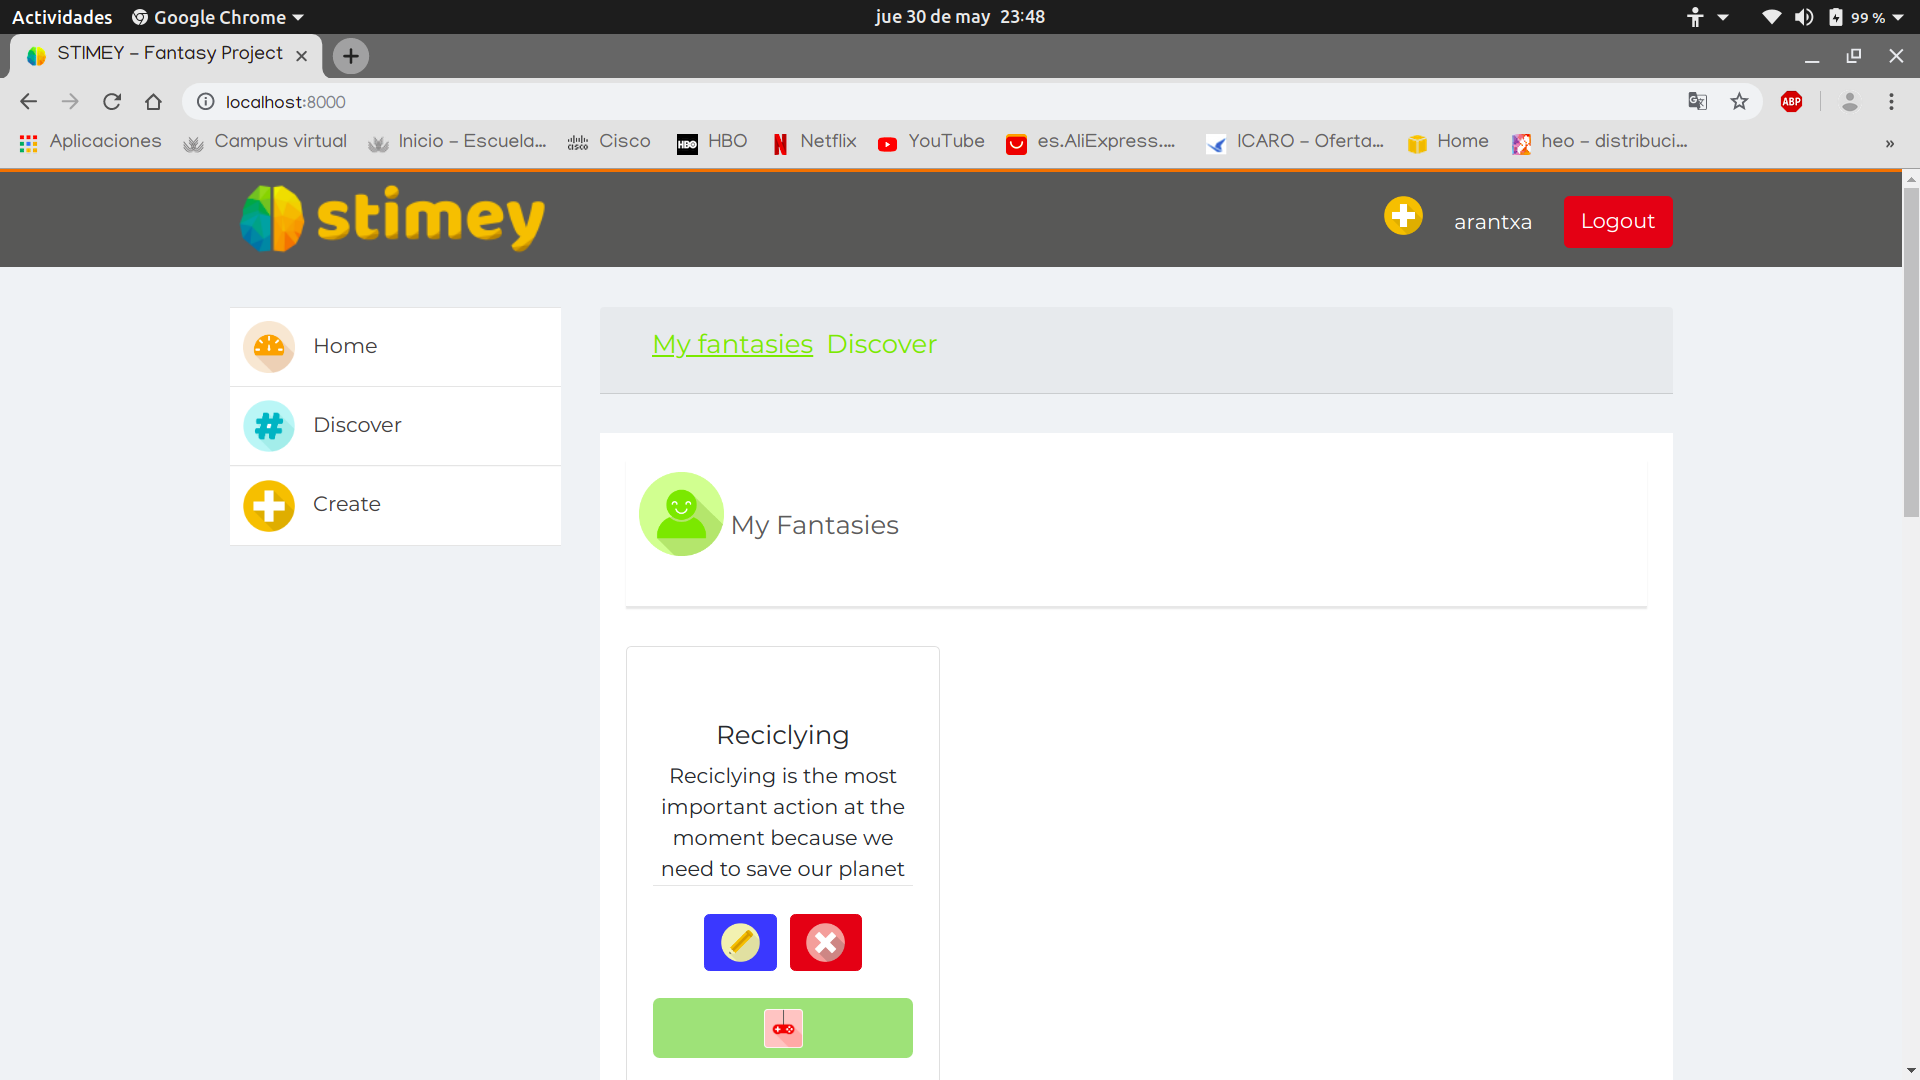
\includegraphics[scale=0.2]{Portada.png}	
  \end{center}
  
\end{frame}

\begin{frame}{Índice}
  \tableofcontents
  % You might wish to add the option [pausesections]
\end{frame}

% Section and subsections will appear in the presentation overview
% and table of contents.

\section{Man-in-the-Middle}
\subsection{Definición}
\begin{frame}{Man-in-the-Middle}
	\begin{block}{Definición}
		Es un ataque donde el atacante puede leer, insertar y modificar los datos recibidos de una víctima a voluntad. Dicho atacante se coloca entre el emisor original del mensaje y el receptor original del mismo sin que ninguno de ellos sepa de la existencia del atacante. Debido a esto, ninguna de las partes sabe que el mensaje enviado/recibido ha sido violado por el atacante.
	\end{block}
	\begin{center}
		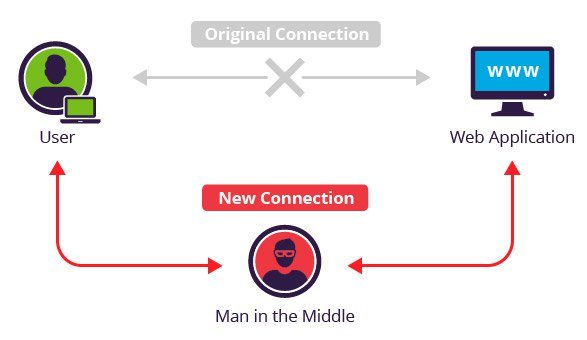
\includegraphics[scale=0.35]{mitm.jpg}
	\end{center}
\end{frame}

\section{Ettercap}
\subsection{Definición}
\begin{frame}{¿Qué es Ettercap?}
	\begin{block}{Definición}
		Es un sniffer para redes LAN que permite la lectura, inyección y modificación de datos en una conexión establecida gracias a un ataque ``Man-in-the-middle''.
	\end{block}
\end{frame}

\subsection{Funcionamiento}
\begin{frame}{¿Cómo funciona Ettercap?}
	\begin{block}{Funcionamiento}
		Para el ejemplo en el que nos vamos a centrar, simplemente usaremos un ataque ``Man-in-the-middle'' para la lectura de las credenciales de usuario en una página web con protocolo HTTP debido a que las páginas que usan HTTPS tienen un cifrado de credenciales y no podemos acceder a dichas credenciales de usuario.
	\end{block}
\end{frame}

\subsection{Ataque práctico con Ettercap}
\begin{frame}{Ejemplo práctico con Ettercap}
	\begin{block}{Requisitos}
		\begin{itemize}
			\item Una red.
			\item Un host usuario.
			\item Un host atacante.
			\item Ettercap.
		\end{itemize}
	\end{block}	
\end{frame}

\section{SSLStrip}
\subsection{Definición}
\begin{frame}{¿Qué es SSLStrip?}
	\begin{block}{Definición}
		Es una aplicación capaz de descifrar el tráfico HTTPS que viaja a través de una red dejándolo visible en "texto plano".
	\end{block}
	\begin{center}
		
\includegraphics[scale=0.75]{https.png}
	\end{center}
\end{frame}

\subsection{¿Cómo funciona SSLStrip?}
\begin{frame}{¿Cómo funciona SSLStrip?}
	\begin{block}{Funcionamiento}
		SSLStrip no descifra el protocolo HTTPS. Su función es engañar al servidor y convertir todo el mensaje HTTPS cifrado de una web en un mensaje HTTP (sin cifrar). Esto solo funciona cuando la víctima llega la página web mediante una redirección o un link.
	\end{block}
\end{frame}

\subsection{Ataque práctico con SSLStrip}
\begin{frame}{Ejemplo práctico con SSLStrip}
	\begin{block}{Requisitos}
		\begin{itemize}
			\item Una red.
			\item Un host usuario.
			\item Un host atacante.
			\item Ettercap.
			\item Script SSLStrip.
		\end{itemize}
	\end{block}	
\end{frame}

\section{HSTS}
\subsection{¿Qué ha pasado?}
\begin{frame}{¿Qué ha pasado?}
	\begin{block}{Resultado del ataque}
		Parece ser que el ataque no ha funcionado sin motivo alguno.
	\end{block}
	\begin{alertblock}{¿Por qué?}
		Debido a que los navegadores hoy día disponen de una contramedida a los sslstrip llamada HSTS.
	\end{alertblock}	
\end{frame}

\subsection{Definición de HSTS}
\begin{frame}{¿Qué es HSTS?}
	\begin{block}{Definición}
		Es un protocolo de seguridad que deniega las conexiones HTTP y solo posibilita las comunicaciones HTTPS entre el cliente y el servidor.
	\end{block}
	\begin{block}{¿Cómo funciona?}
		 Para poder activar esta utilidad, el usuario debe ser capaz de haber establecido una conexión al menos una vez de forma exitosa con dicha web.
	\end{block}
\end{frame}

\end{document}


